% Auriga theme
% https://github.com/anishathalye/auriga

\documentclass[14pt,aspectratio=169]{beamer}
\usepackage{pgfpages}
\usepackage{fancyvrb}
\usepackage{tikz}
\usepackage{pgfplots}
\usepackage{graphicx}
\usepackage{amsmath}

%\ifnotes
%\setbeamertemplate{note page}[plain]
%\setbeameroption{show notes on second screen=right}
%\fi

\usetheme{auriga}
\usecolortheme{auriga}

% define some colors for a consistent theme across slides
\definecolor{red}{RGB}{181, 23, 0}
\definecolor{blue}{RGB}{0, 118, 186}
\definecolor{gray}{RGB}{146, 146, 146}
\definecolor{yelow}{RGB}{255, 205, 0}

\title{Waveguide propagation}

\author{\underline{Ime Rasenberg} \inst{1} \and \underline{Bram Jan Spijkerman} \inst{1}}

\institute[shortinst]{\inst{1} Utrecht Universiteit}

\begin{document}

{
  % rather than use the frame options [noframenumbering,plain], we make the
  % color match, so that the indicated page numbers match PDF page numbers
  \setbeamercolor{page number in head/foot}{fg=white}
  \begin{frame}
    \titlepage
  \end{frame}
}

\input{slides/bullets}
\input{slides/split}
\begin{frame}{WHY NO WORK}

  \begin{minipage}{0.55\textwidth}
    \begin{align*}
      \frac{\omega}{c} &= \sqrt{k_x^2+\left(\frac{m\pi}{L}\right)^2}\\\\
      \phi_{in}(z) &= C_1\phi_1(z) + C_2\phi_2(z)\\\\
      C_i &= \int_{-\infty}^{\infty}dz\,\phi_{in}(z)\phi_i(z)
    \end{align*}
  \end{minipage}\hfill
  \begin{minipage}{0.4\textwidth}
  \begin{figure}
    \centering
    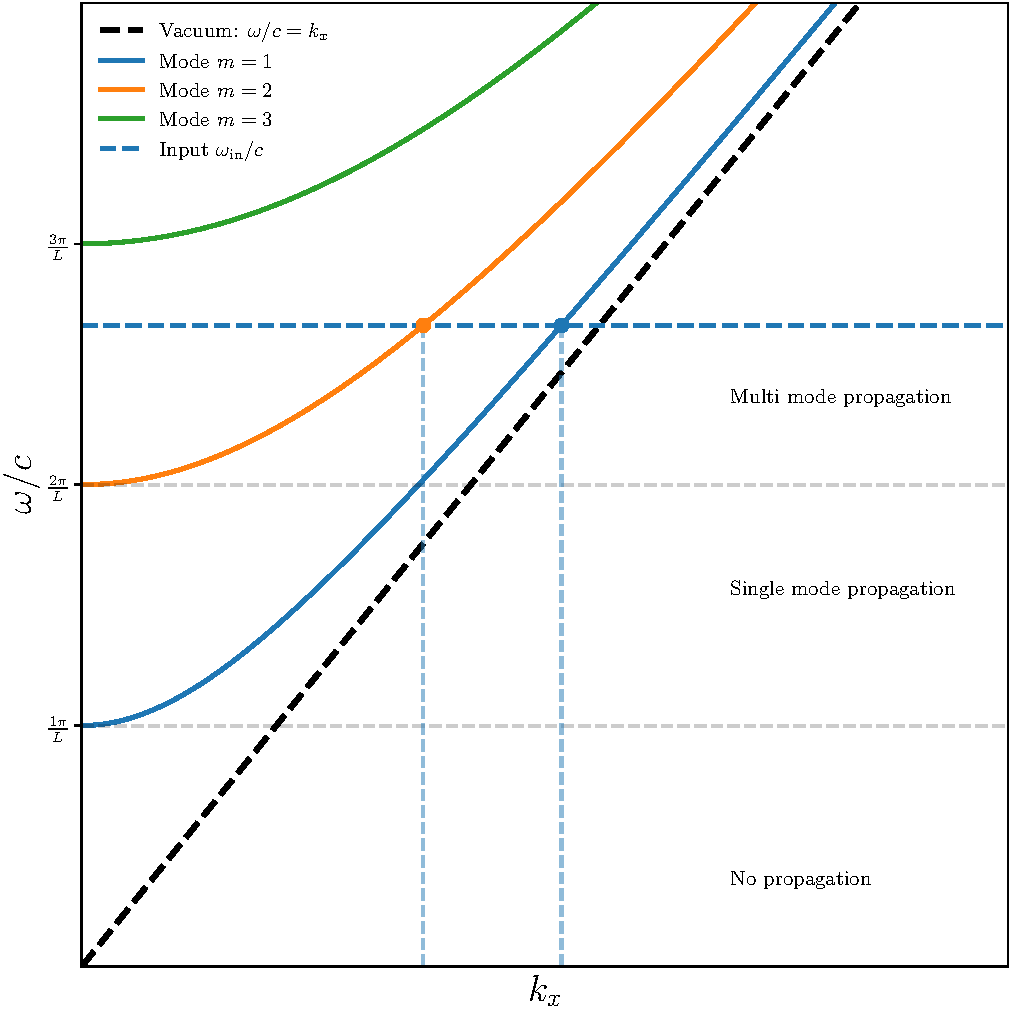
\includegraphics[width=\textwidth]{img/dispersion_diagram.pdf}
    \caption{The figure's caption}
  \end{figure}
  \end{minipage}
\end{frame}

\input{slides/centered}
\input{slides/monospace}
\input{slides/brackets}
\input{slides/link}

\end{document}
